%!TEX root = da-screen.tex

So far we have studied deterministic distributed algorithms in port-numbered networks. Now we will introduce another model of distributed computing: deterministic distributed algorithms in \emph{networks with unique identifiers}. Following the standard terminology of the field, we will use the term ``$\LOCAL$ model'' to refer to networks with unique identifiers.


\section{Introduction}

In the $\LOCAL$ model, we assume that we are given a node labelling $\Id\colon V \to \NN$ such that each node $v$ has a unique label~$\Id(v)$; see Figure~\ref{fig:unique-ids} for an example. We will assume that the labels are reasonably small\mydash in an $n$-node network, the labels are $O(\log n)$-bit integers.

\begin{figure}
    \centering
    \includegraphics[page=\PUniqueIds]{figs.pdf}
    \caption{A network with unique identifiers.}\label{fig:unique-ids}
\end{figure}

As such, the model does not seem to be a major deviation from what we have studied so far. We have already encountered various extensions of the port-numbering model\mydash for example, we have studied distributed algorithms that assume that we are given a colouring of the nodes or an orientation of the edges.

However, once we have unique identifiers, we can no longer apply techniques based on covering graphs (see Chapter~\ref{ch:covering-map}) to prove impossibility results. It turns out that \emph{any} computable graph problem on connected graphs can be solved if we are given unique identifiers. Hence we are no longer interested in what can be solved; the key question is what can be solved \emph{fast}.


\section{Networks with Unique Identifiers}

There are plenty of examples of real-world networks with globally unique identifiers: public IPv4 and IPv6 addresses are globally unique identifiers of Internet hosts, devices connected to an Ethernet network have globally unique MAC addresses, mobile phones have their IMEI numbers, etc.

The common theme is that the identifiers are (supposed to be) globally unique, and the numbers can be interpreted as natural numbers. Moreover, the numbers are relatively small but not as small as possible: in a network with millions of devices we may have allocated a space of billions of possible identifiers. In particular, there is no guarantee that a device with identifier ``1'' exists in the network at any given time.

We will now give the formal definition that aims at capturing these properties of real-world networks.


\section{Definition of the \tLOCAL{} Model}\label{sec:unique-id}

Throughout this chapter, fix a constant $c > 1$. \emph{Unique identifiers} for a port-numbered network $N = (V,P,p)$ is an injection
\[
    \Id \colon V \to \{1,2, \dotsc, |V|^c\}.
\]
That is, each node $v \in V$ is labelled with a unique integer, and the labels are assumed to be relatively small (in comparison with the number of nodes in network $N$).

Formally, unique identifiers can be interpreted as a graph problem $\Pi'$, where each solution $\Id \in \Pi'(N)$ is an assignment of unique identifiers for network $N$. If a distributed algorithm $A$ solves a problem $\Pi$ on a family $\calF$ given $\Pi'$, we say that $A$ solves $\Pi$ on $\calF$ \emph{given unique identifiers}, or equivalently, $A$ solves $\Pi$ on $\calF$ \emph{in the model of unique identifiers}.

For the sake of convenience, when we discuss networks with unique identifiers, we will assume that
\[
    v = \Id(v) \text{ for all } v \in V.
\]
Put otherwise, we assume that the set $V$ is a subset of natural numbers, and $\max V \le |V|^c$.


\section{Gathering Everything}\label{sec:gather}

In the model of unique identifiers, if the underlying graph $G = (V,E)$ is connected, all nodes can learn everything about $G$ in time $O(\diam(G))$. In this section, we will present algorithm $\algo{Gather}$ that accomplishes this.

In algorithm $\algo{Gather}$, each node $v \in V$ will construct sets $V(v,r)$ and $E(v,r)$, where $r = 1, 2, \dotsc$. For all $v \in V$ and $r \ge 1$, these sets will satisfy
\begin{align}
    V(v,r) &= \ball_G(v,r), \label{eq:gather1} \\
    E(v,r) &= \bigl\{ \{s,t\} : s \in \ball_G(v,r),\, t\in \ball_G(v,r{-}1) \bigr\}. \label{eq:gather2}
\intertext{Now define the graph}
    G(v,r) &= (V(v,r), E(v,r)).  \label{eq:gather3}
\end{align}
See Figure~\ref{fig:gather} for an illustration.

\begin{figure}
    \centering
    \includegraphics[page=\PGather]{figs.pdf}
    \caption{Subgraph $G(v,r)$ defined in \eqref{eq:gather3}, for $v = 14$ and $r = 2$.}\label{fig:gather}
\end{figure}

The following properties are straightforward corollaries of \eqref{eq:gather1}--\eqref{eq:gather3}.
\begin{enumerate}
    \item Graph $G(v,r)$ is a subgraph of $G(v,r+1)$, which is a subgraph of $G$.
    \item If $G$ is a connected graph, and $r \ge \diam(G) + 1$, we have $G(v,r) = G$.
    \item More generally, if $G_v$ is the connected component of $G$ that contains $v$, and $r \ge \diam(G_v) + 1$, we have $G(v,r) = G_v$.
    \item For a sufficiently large $r$, we have $G(v,r) = G(v,r+1)$.
    \item If $G(v,r) = G(v,r+1)$, we will also have $G(v,r+1) = G(v,r+2)$.
    \item Graph $G(v,r)$ for $r > 1$ can be constructed recursively as follows:
    \begin{align}
        V(v,r) &= \bigcup_{u \in V(v,1)} V(u,r-1), \label{eq:Vvr} \\
        E(v,r) &= \bigcup_{u \in V(v,1)} E(u,r-1). \label{eq:Evr}
    \end{align}
\end{enumerate} 

Algorithm $\algo{Gather}$ maintains the following invariant: after round $r \ge 1$, each node $v \in V$ has constructed graph $G(v,r)$. The execution of $\algo{Gather}$ proceeds as follows:
\begin{enumerate}
    \item In round $1$, each node $u \in V$ sends its identity $u$ to each of its ports. Hence after round $1$, each node $v \in V$ knows its own identity and the identities of its neighbours. Put otherwise, $v$ knows precisely $G(v,1)$.
    \item In round $r > 1$, each node $u \in V$ sends $G(u,r-1)$ to each of its ports. Hence after round $r$, each node $v \in V$ knows $G(u,r-1)$ for all $u \in V(v,1)$. Now $v$ can reconstruct $G(v,r)$ using \eqref{eq:Vvr} and \eqref{eq:Evr}.
    \item A node $v \in V$ can stop once it detects that the graph $G(v,r)$ no longer changes.
\end{enumerate}

It is straightforward to extend $\algo{Gather}$ so that we can discover not only the underlying graph $G = (V,E)$ but also the original port-numbered network $N = (V,P,p)$.


\section{Solving Everything}

Let $\calF$ be a family of connected graphs, and let $\Pi$ be a distributed graph problem. Assume that there is a deterministic \emph{centralised} (non-distributed) algorithm $A'$ that solves $\Pi$ on $\calF$. For example, $A'$ can be a simple brute-force algorithm\mydash we are not interested in the running time of algorithm~$A'$.

Now there is a simple distributed algorithm $A$ that solves $\Pi$ on $\calF$ in the model of unique identifiers. Let $N = (V,P,p)$ be a port-numbered network with the underlying graph $G \in \calF$. Algorithm $A$ proceeds as follows.
\begin{enumerate}
    \item All nodes discover $N$ using algorithm $\algo{Gather}$ from Section~\ref{sec:gather}.
    \item All nodes use the centralised algorithm $A'$ to find a solution $f \in \Pi(N)$. From the perspective of algorithm $A$, this is merely a state transition; it is a local step that requires no communication at all, and hence takes $0$ communication rounds.
    \item Finally, each node $v \in V$ switches to state $f(v)$ and stops.
\end{enumerate}
Clearly, the running time of the algorithm is $O(\diam(G))$.

It is essential that all nodes have the same canonical representation of network $N$ (for example, $V$, $P$, and $p$ are represented as lists that are ordered lexicographically by node identifiers and port numbers), and that all nodes use the same deterministic algorithm $A'$ to solve $\Pi$. This way we are guaranteed that all nodes have locally computed the \emph{same} solution $f$, and hence the outputs $f(v)$ are globally consistent.


\section{Focus on Complexity}

The above discussion highlights the striking difference between the port-numbering model and the model of unique identifiers. While there are plenty of examples of graph problems that cannot be solved at all in the port-numbering model, with the help of unique identifiers all computable graph problems become solvable.

Hence our focus shifts from computability to computational complexity. While it is trivial to determine if a problem can be solved in the model of unique identifiers, we would like to know which problems can be solved quickly. In particular, we would like to learn which problems can be solved in time that is much smaller than $\diam(G)$. One such problem is graph colouring.


\section{Graph Colouring}

Let $G = (V,E)$ be a graph with unique identifiers. We will use the shorthand notation $\chi = |V|^c$, that is, the unique identifiers are integers from $\{1,2,\dotsc,\chi\}$.

The unique identifiers form a proper vertex colouring with $\chi$ colours: certainly adjacent nodes have distinct identifiers if the identifiers are globally unique. Hence, in a sense, we have already solved the graph colouring problem\mydash however, the number of colours $\chi$ is far too large for our purposes.

Our focus is therefore on \emph{colour reduction}: given a graph colouring $f\colon V \to \{1,2,\dotsc,x\}$ with a large number $x$ of colours, the goal is to find a new graph colouring $g\colon V \to \{1,2,\dotsc,y\}$ with a smaller number $y < x$ of colours.


\subsection{Greedy Colour Reduction}\label{ssec:greedy}

Let $x \in \NN$. There is a simple algorithm $\algo{Greedy}$ that reduces the number of colours from $x$ to
\[
    y = \max \{ x-1, \Delta+1 \},
\]
where $\Delta$ is the maximum degree of the graph. The running time of the algorithm is one communication round.

The algorithm proceeds as follows; here $f$ is the $x$-colouring that we are given as input and $g$ is the $y$-colouring that we produce as output. See Figure~\ref{fig:greedy} for an illustration.
\begin{enumerate}
    \item In the first communication round, each node $v \in V$ sends its colour $f(v)$ to each of its neighbours.
    \item Now each node $v \in V$ knows the set
    \[
        C(v) = \{ i : \text{there is a neighbour $u$ of $v$ with $f(u) = i$} \}.
    \]
    We say that a node is \emph{active} if $f(v) > \max C(v)$; otherwise it is \emph{passive}. That is, the colours of the active nodes are local maxima. Let
    \[
        \bar{C}(v) = \{1,2,\dotsc\} \setminus C(v)
    \]
    be the set of \emph{free colours} in the neighbourhood of $v$.
    \item A node $v \in V$ outputs
    \[
        g(v) = \begin{cases}
            f(v) & \text{if $v$ is passive}, \\
            \min \bar{C}(v) & \text{if $v$ is active}.
        \end{cases}
    \]
\end{enumerate}
Informally, a node whose colour is a local maximum re-colours itself with the first available free colour.

\begin{figure}
    \centering
    \includegraphics[page=\PGreedy]{figs.pdf}
    \caption{Greedy colour reduction. The active nodes have been highlighted. In this example, each active node can choose $1$ as its new colour. Note that in the original colouring $f$, the largest colour was $99$, while in the new colouring, the largest colour is strictly smaller than $99$\mydash we successfully reduced the number of colours in the graph.}\label{fig:greedy}
\end{figure}

\begin{lemma}
    Algorithm \algo{Greedy} reduces the number of colours from $x$ to
    \[
        y = \max \{ x-1, \Delta+1 \},
    \]
    where $\Delta$ is the maximum degree of the graph.
\end{lemma}
\begin{proof}
    Let us first prove that $g(v) \in \{1,2,\dotsc,y\}$ for all $v \in V$. As $f$ is a proper colouring, we cannot have $f(v) = \max C(v)$. Hence there are only two possibilities.
    \begin{enumerate}
        \item $f(v) < \max C(v)$. Now $v$ is passive, and it is adjacent to a node $u$ such that $f(v) < f(u)$. We have
        \[
            g(v) = f(v) \le f(u) - 1 \le x - 1 \le y.
        \]
        \item $f(v) > \max C(v)$. Now $v$ is active, and we have
        \[
            g(v) = \min \bar{C}(v).
        \]
        There is at least one value $i \in \{1,2,\dotsc,|C(v)|+1\}$ with $i \notin C(v)$; hence
        \[
            \min \bar{C}(v) \le |C(v)| + 1 \le \deg_G(v) + 1 \le \Delta + 1 \le y.
        \]
    \end{enumerate}
    
    Next we will show that $g$ is a proper vertex colouring of $G$. Let $\{u,v\} \in E$. If both $u$ and $v$ are passive, we have
    \[
        g(u) = f(u) \ne f(v) = g(v).
    \]
    Otherwise, w.l.o.g., assume that $u$ is active. Then we must have $f(u) > f(v)$. It follows that $f(u) \in C(v)$ and $f(v) \le \max C(v)$; therefore $v$ is passive. Now
    $g(u) \notin C(u)$ while
    $g(v) = f(v) \in C(u)$; we have $g(u) \ne g(v)$.
\end{proof}

A key observation in understanding the algorithm is that the set of active nodes forms an independent set. Therefore all active nodes can pick their new colours simultaneously in parallel, without any risk of choosing colours that might conflict with each other.

Note that algorithm $\algo{Greedy}$ does not need to know the number of colours $x$ or the maximum degree $\Delta$; we only used them in the analysis. We can simply take any graph, blindly apply algorithm $\algo{Greedy}$, and we are guaranteed to reduce the number of colours by one\mydash provided that the number of colours was larger than $\Delta + 1$.

In particular, we can apply algorithm $\algo{Greedy}$ repeatedly until we get stuck, at which point we have a \Dpocol{} of~$G$\mydash we will formalise and generalise this idea in Exercise~\ref{ex:greedy-iterate}.

In principle, we could use this strategy in the model of unique identifiers to find a \Dpocol{} of any graph. However, such an algorithm would be extremely slow. In the worst case, we may have a long path of nodes, with increasing identifiers (colours) along the path, and in such a graph the running time of the greedy strategy would be linear in $|V|$: in each iteration, only one of the nodes is a local maximum.

In the next sections, we will develop an algorithm that is much faster\mydash at least in low-degree graphs.


\subsection{Directed Pseudoforests}

We will first study fast colour reduction algorithms in a seemingly simple special case: we are given a pseudoforest with a particular orientation. Once we have solved the special case, we turn our attention to the more general case of colouring bounded-degree graphs.

A \emph{directed pseudoforest} is a directed graph $G = (V,E)$ such that each node $v \in V$ has $\outdegree_G(v) \le 1$; see Figure~\ref{fig:dp} for an example. We make the following observations:
\begin{enumerate}
    \item Let $H$ be an undirected graph, and let $G$ be an orientation of $H$. If $G$ is a directed pseudoforest, then $H$ is a pseudoforest.
    \item Let $H$ be a pseudoforest. There exists an orientation $G$ of $H$ such that $G$ is a directed pseudoforest.
    \item An orientation of a pseudoforest is not necessarily a directed pseudoforest.
\end{enumerate}
If $(u,v) \in E$, we say that $v$ is a \emph{successor} of $u$ and $u$ is a \emph{predecessor} of $v$. By definition, in a directed pseudoforest each node has at most one successor.

\begin{figure}
    \centering
    \includegraphics[page=\PDP]{figs.pdf}
    \caption{A directed pseudoforest with a colouring~$f$.}\label{fig:dp}
\end{figure}

\subsection{Greedy Colouring in Pseudoforests}\label{ssec:dpgreedy}

We will soon see that we can do colour reduction in directed pseudoforests quickly. However, let us first show that we can find a colouring with a very small number of colours with a modified version of algorithm $\algo{Greedy}$.

Let $G = (V,E)$ be a directed pseudoforest, and let \[f\colon V \to \{1,2,\dotsc,x\}\] be a proper vertex colouring of $G$, for some $x \ge 4$. We design a distributed algorithm $\algo{DPGreedy}$ that reduces the number of colours from $x$ to $x-1$ in two communication rounds.

First, for each node $v \in V$, define $s(v)$ as follows:
\begin{enumerate}
    \item If $\outdegree_G(v) = 1$, let $u$ be the successor of $v$, and let $s(v) = f(u)$.
    \item Otherwise, if $f(v) > 1$, let $s(v) = 1$.
    \item Otherwise $s(v) = 2$.
\end{enumerate}
By construction, we have $s(v) \ne f(v)$. Note that we can compute the values $s(v)$ for all nodes $v \in V$ with a simple distributed algorithm in one communication round.

\begin{figure}
    \centering
    \includegraphics[page=\PDPSuccessor]{figs.pdf}
    \caption{A directed pseudoforest with colouring~$s$; compare with Figure~\ref{fig:dp}. In colouring $s$, all predecessors of a node have the same colour; hence each node is adjacent to nodes of only two different colours.}\label{fig:dpsuccessor}
\end{figure}

We will now prove that the values $s(v)$ form a proper $x$-colouring of $G$. Moreover, we show that each node is adjacent to only two different colours in colouring~$s$.

\begin{lemma}
    Function $s$ is an $x$-colouring of $G$.
\end{lemma}
\begin{proof}
    By construction, we have $s(v) \in \{1,2,\dotsc,x\}$.
    
    Now let $(u,v) \in E$. We need to show that $s(u) \ne s(v)$. To see this, observe that $v$ is a successor of $u$. Hence
    \[
        s(u) = f(v) \ne s(v). \qedhere
    \]
\end{proof}

\begin{lemma}
    Define
    \[
        C(v) = \{ i : \text{there is a neighbour $u$ of $v$ with $s(u) = i$} \}.
    \]
    We have $|C(v)| \le 2$ for each node $v \in V$.
\end{lemma}
\begin{proof}
    For each predecessor $u$ of $v$, we have $s(u) = f(v)$. That is, all predecessors of $v$ have the same colour. Hence $C(v)$ consists of at most two different values: the common colour of the predecessors of $v$ (if any), and the colour of the successor of $v$ (if any).
\end{proof}

Now we apply algorithm $\algo{Greedy}$ to colouring $s$; see Figure~\ref{fig:dpgreedy}. Observe that each active node $v$ will choose a colour $g(v) = \min \bar{C}(v) \in \{1,2,3\}$, while each passive node $v$ will output its old colour $g(v) = s(v)$. In particular, if the number of colours in $f$ was $x \ge 4$, then the number of colours in $g$ is at most $x - 1$.

\begin{figure}
    \centering
    \includegraphics[page=\PDPGreedy]{figs.pdf}
    \caption{Algorithm $\algo{Greedy}$ applied to a directed pseudoforest with colouring~$s$. The active nodes are highlighted.}\label{fig:dpgreedy}
\end{figure}

Let us summarise the above observations. We have designed algorithm $\algo{DPGreedy}$ that reduces the number of colours from $x \ge 4$ to $x-1$ in directed pseudoforests in $2$ communication rounds:
\begin{enumerate}
    \item We are given an $x$-colouring $f$ (Figure~\ref{fig:dp}).
    \item In one communication round, given $f$ we construct another $x$-colouring $s$, which has the property that each node is adjacent to at most two different colour classes (Figure~\ref{fig:dpsuccessor}).
    \item In one communication round, given $s$ we construct an $(x-\nobreak 1)$-colouring $g$ using algorithm $\algo{Greedy}$ (Figure~\ref{fig:dpgreedy}).
\end{enumerate}
In particular, we can reduce the number of colours from any number $x \ge 3$ to $3$ in ${2(x-3)}$ rounds by iterating the above steps.

Figure~\ref{fig:dpcritical} demonstrates that the additional step of constructing colouring $s$ is necessary.

\begin{figure}
    \centering
    \includegraphics[page=\PDPCritical]{figs.pdf}
    \caption{(a)~If we tried to apply algorithm $\algo{Greedy}$ directly in any given colouring $f$, the active nodes would not be able to pick new colours from the set $\{1,2,3\}$. (b)~In colouring $s$, algorithm $\algo{Greedy}$ will always find a new colour from the set $\{1,2,3\}$.}\label{fig:dpcritical}
\end{figure}

\subsection{Fast Colouring in Pseudoforests}\label{ssec:dpbit}

So far we have only seen algorithms that reduce the number of colours by one in each iteration. This is by far too slow if, for example, we are given a colouring that is formed by $128$-bit IPv6 addresses. In this section we will present an algorithm that is \emph{much} faster.

In particular, we present algorithm $\algo{DPBit}$ that reduces the number of colours from $2^x$ to $2x$ in one communication round, in any directed pseudoforest. We will assume that $x \ge 1$ is a known constant.

Before presenting algorithm $\algo{DPBit}$, we will give a practical example of its performance. Assume that the initial colouring is derived from $128$-bit unique identifiers, that is, the number of colours is $2^{128}$. If we iterate algorithm $\algo{DPBit}$, we can reduce the number of colours as follows:
\begin{align*}
    2^{128} &\to 2 \cdot 128 = 2^8, \\
    2^8 &\to 2 \cdot 8 = 2^4, \\
    2^4 &\to 2 \cdot 4 = 2^3, \\
    2^3 &\to 2 \cdot 3 = 6.
\end{align*}
That is, given a $2^{128}$-colouring, in only $4$ communication rounds, we can find a $6$-colouring. We cannot reduce the number of colours below $6$ with $\algo{DPBit}$; however, once we have reached such a low number of colours, we can resort to $\algo{DPGreedy}$, which is able to reduce the number of colours from $6$ to $3$ in $6$ communication rounds. In summary, we can reduce the number of colours from $2^{128}$ to $3$ in only $4+6 = 10$ rounds, in any directed pseudoforest.

Let us now present algorithm $\algo{DPBit}$. We assume that we are given a proper vertex colouring
\[
    f \colon V \to \{ 1,2,\dotsc,2^x\}
\]    
of a directed pseudoforest $G = (V,E)$. We will use the values $s(v)$ defined in Section~\ref{ssec:dpgreedy}\mydash recall that $f(v) \ne s(v)$ for each node $v$, and if $u$ is the successor of $v$, we have $s(v) = f(u)$.

The key idea is that each node compares the \emph{binary encodings} of the values $s(v)$ and $f(v)$. More precisely, if $j \in \{1,2,\dotsc,2^x\}$ is a colour, let us use $\bin{j}$ to denote the binary encoding of $j-1$; this is always a binary string of length $x$. For example, if $x = 3$, we have
\[
    \bin{1} = 000,\quad
    \bin{2} = 001,\quad
    \dotsc, \quad
    \bin{8} = 111.
\]
If $i \in \{0,1,\dotsc,x-1\}$, we use the notation $\bin{j}_i$ to refer to bit $i$ of the binary string $\bin{j}$, counting from the lowest-order bit. For example, $\bin{2}_0 = 1$ and $\bin{2}_1 = 0$.

In algorithm $\algo{DPBit}$, each node first finds out the values $s(v)$ and $f(v)$\mydash this takes only one communication round\mydash and then compares the binary strings $\bin{s(v)}$ and $\bin{f(v)}$. As $s(v) \ne f(v)$, there is at least one bit in these strings that differs. Let
\[
    i(v) = \min \{ i : \bin{f(v)}_i \ne \bin{s(v)}_i \}
\]
be the \emph{index} of the first bit that differs, and let
\[
    b(v) = \bin{f(v)}_{i(v)}
\]
be the \emph{value} of the bit that differs. Note that $0 \le i(v) \le x-1$ and $0 \le b(v) \le 1$.

The key observation is that the pairs $\bigl(i(v), b(v)\bigr)$ form a proper colouring of $G$.
\begin{lemma}\label{lem:dpbit}
    Let $(u,v) \in E$. We have $i(u) \ne i(v)$ or $b(u) \ne b(v)$.
\end{lemma}
\begin{proof}
    If $i(u) \ne i(v)$, the claim is trivial. Otherwise $i(u) = i(v)$. As $v$ is the successor of $u$, we have $s(u) = f(v)$. Hence
    \begin{align*}
        b(v) &= \bin{f(v)}_{i(v)} = \bin{s(u)}_{i(u)}, \\
    \intertext{and by the definition of $i(u)$,}
        b(u) &= \bin{f(u)}_{i(u)} \ne \bin{s(u)}_{i(u)}.
    \end{align*}
    In summary, $b(u) \ne b(v)$.
\end{proof}

We can now encode the pair $\bigl(i(v), b(v)\bigr)$ as a colour
\[
    g(v) = 2i(v) + b(v) + 1.
\]
Algorithm $\algo{DPBit}$ outputs the value $g(v)$.

Note that if we have $g(u) = g(v)$ for two nodes $u$ and $v$, this implies $b(u) = b(v)$ and $i(u) = i(v)$. Hence Lemma~\ref{lem:dpbit} implies that $g$ is a proper vertex colouring of $G$. Moreover, we have $1 \le g(v) \le 2x$, and hence $g$ is a $2x$-colouring of $G$.

In summary, we have designed algorithm $\algo{DPBit}$ that reduces the number of colours from $2^x$ to $2x$ in one communication round\mydash given a $2^x$-colouring $f$, the algorithm outputs a $2x$-colouring $g$. Communication is only needed in order to discover the value $s(v)$ for each node $v$; the derivation of the values $i(v)$, $b(v)$, and $g(v)$ only needs local computation.


\subsection{Fast Colouring in General Graphs}\label{ssec:colour}

In this section, we will present algorithm $\algo{Colour}$ that reduces the number of colours from any number $x$ to $\Delta+1$ in any graph of maximum degree at most $\Delta$ much faster than an iterated application of algorithm $\algo{Greedy}$. Throughout this section, we will assume that the values of $x$ and $\Delta$ are known to all nodes.

Let $A$ be an algorithm that reduces the number of colours in a directed pseudoforest from $x$ to $3$ in time $T(x)$. For example, we can let $A$ be the combination of the iterated $\algo{DPBit}$ (reduces the number of colours from any $x$ to $6$) followed by the iterated $\algo{DPGreedy}$ (reduces the number of colours from $6$ to $3$). As we will see in Exercise~\ref{ex:logstar}, the running time of $A$ is then $T(x) = O(\log^* x)$.

Algorithm $\algo{Colour}$ uses $A$ as a subroutine, and the running time of $\algo{Colour}$ will be $O(\Delta^2) + T(x)$. For example, with the above choice of $A$, the running time of $\algo{Colour}$ is $O(\Delta^2 + \log^* x)$.

Let $G = (V,E)$ be a graph of maximum degree at most $\Delta$, and let $f \colon V \to \{1,2,\dotsc,x\}$ be an $x$-colouring of $G$. Let $N$ be a port-numbered network with $G$ as the underlying graph. Algorithm $\algo{Colour}$ constructs a \Dpocol{} $g$ of $G$ as follows.

\paragraph{Preliminaries.}

For each node $v$ and each port number $i$, node $v$ sends the pair $(f(v), i)$ to port $i$. This way a node $u$ learns the following information about each node $v$ that is adjacent to~$u$: what is the old colour of $v$, which port of $u$ is connected to $v$, and which port of $v$ is connected to $u$. This step requires one communication round.

\paragraph{Orientation.}

We construct an orientation $G' = (V,E')$ of $G$ as follows: we have $(u,v) \in E'$ if and only if $\{u,v\} \in E$ and $f(u) < f(v)$. That is, we use the old colours of the nodes to orient the edges from a smaller colour to a larger colour; see Figure~\ref{fig:id-orient}.

\begin{figure}
    \centering
    \includegraphics[page=\PIdOrient]{figs.pdf}
    \caption{Orientation $G'$ derived from the old colours\mydash in this example, the old colours were unique identifiers.}\label{fig:id-orient}
\end{figure}

In the distributed algorithm, each node only needs to know the orientation of its incident edges. This step requires zero communication rounds.

\paragraph{Partition in Pseudoforests.}

For each $i = 1,2,\dotsc,\Delta$, we construct a subgraph $G_i = (V,E_i)$ of $G'$ as follows: we have $(u,v) \in E_i$ if and only if $(u,v) \in E'$ and $v$ is connected to port number $i$ of $u$ in $N$. See Figure~\ref{fig:id-pick-class}.

\begin{figure}
    \centering
    \includegraphics[page=\PIdPickClass]{figs.pdf}
    \caption{Subgraph $G_i$ of $G'$. Each node has outdegree at most one.}\label{fig:id-pick-class}
\end{figure}
    
Observe that the sets $E_1, E_2, \dotsc, E_\Delta$ form a partition of $E'$: for each directed edge $e \in E'$ there is precisely one $i$ such that $e \in E_i$. Also note that for each node $u \in V$ and for each index $i$ there is at most one neighbour $v$ such that $(u,v) \in E_i$. It follows that the outdegree of any node $v$ in $G_i = (V,E_i)$ is at most one, and therefore $G_i$ is a \emph{directed pseudoforest}. Function $f$ is an $x$-colouring of $G_i$ for all $i$.
    
In the distributed algorithm, each node only needs to know which of its incident edges are in which subset $E_i$. This step requires zero communication rounds.

\paragraph{Parallel Colouring of Pseudoforests.}

For each $i$, we use algorithm $A$ to construct a $3$-colouring $g_i$ of $G_i$.
    
In the distributed algorithm, each node $v \in V$ needs to know the value $g_i(v)$ for each $i$. This step takes only $T(x)$ rounds: we can simulate the execution of $A$ in parallel for all subgraphs $G_i$. In the simulation, each node has $\Delta$ different roles, one for each subgraph $G_i$.

\paragraph{Merging Colourings.}

For each $j = 0, 1, \dotsc, \Delta$, define
\[
    E'_j = \bigcup_{i = 1}^j E_i
\]
and $G'_j = (V,E'_j)$. Note that $G'_0$ is a graph without any edges, each $G'_j$ is a subgraph of $G'$, and $G'_\Delta = G'$.

We will construct a sequence of colourings $g'_0, g'_1, \dotsc, g'_\Delta$ such that $g'_j$ is a \Dpocol{} of the subgraph $G'_j$. Then it follows that we can output $g = g'_\Delta$, which is a \Dpocol{} of $G'$ and hence also a \Dpocol{} of the original graph~$G$.

Our construction is recursive. The base case of $j = 0$ is trivial: we can choose $g'_0(v) = 1$ for all $v \in V$, and this is certainly a proper \Dpocol{} of $G'_0$.

Now assume that we have already constructed a \Dpocol{} $g'_{j-1}$ of $G'_{j-1}$. Recall that $g_j$ is a $3$-colouring of $G_j$; see Figure~\ref{fig:merge-colours}. Define a function $h_j$ as follows:
\[
    h_j(v) = (\Delta+1) (g_j(v)-1) + g'_{j-1}(v).
\]
Observe that $h_j$ is a proper $3(\Delta+\nobreak 1)$-colouring of $G'_j$. To see this, consider an edge $(u,v) \in E'_j$. If $(u,v) \in E_j$, we have $g_j(u) \ne g_j(v)$, which implies $h_j(u) \ne h_j(v)$. Otherwise $(u,v) \in E'_{j-1}$, and we have $g'_{j-1}(u) \ne g'_{j-1}(v)$, which implies $h_j(u) \ne h_j(v)$.

\begin{figure}
    \centering
    \includegraphics[page=\PMergeColours]{figs.pdf}
    \caption{Merging a $3$-colouring $g_j$ of directed pseudotree $G_j$ and a \Dpocol{} $g'_{j-1}$ of subgraph $G'_{j-1}$. The end result is a proper $3(\Delta\nobreak +1)$-colouring $h_j$ of subgraph $G'_j$.}\label{fig:merge-colours}
\end{figure}

Now we use $2(\Delta+\nobreak 1)$ iterations of $\algo{Greedy}$ to reduce the number of colours from $3(\Delta+\nobreak 1)$ to $\Delta+\nobreak 1$. This way we can construct a proper \Dpocol{} $g'_j$ of $G'_j$ in time $O(\Delta)$.

After $\Delta$ phases, we have eventually constructed colouring $g = g'_\Delta$; the total running time is $O(\Delta^2)$, as each phase takes $O(\Delta)$ communication rounds.


\section{Exercises}

\begin{ex}[counting]
    The \emph{counting problem} $\Pi$ is defined as follows: if $N = (V,P,p)$ is a port-numbered network, then $g \in \Pi(N)$ if and only if $g(v) = |V|$ for all $v \in V$. That is, in the counting problem each node has to output the value $|V|$, i.e., it has to indicate how many nodes there are in the network.
    
    Let $\calF$ consist of all cycle graphs, and let $\calF'$ consist of all graphs of maximum degree~$2$.
    \begin{subex}
        \item Prove that the counting problem cannot be solved on $\calF$ in the port-numbering model.
        \item Design an algorithm that solves the counting problem on $\calF$ in the model of unique identifiers in time $O(|V|)$. Present the algorithm in a formally precise manner, using the definitions of Sections \ref{sec:pnn} and \ref{sec:distr-alg}.
        \item Prove that the counting problem cannot be solved in time $o(|V|)$ on $\calF$ in the model of unique identifiers.
        \item Prove that the counting problem cannot be solved on $\calF'$ in the model of unique identifiers.
    \end{subex}
\end{ex}

\begin{ex}[leader election]
    The \emph{leader election problem} $\Pi$ is defined as follows: if $N = (V,P,p)$ is a port-numbered network, then $g \in \Pi(N)$ if and only if there is precisely one node $u \in V$ such that
    \[
        g(v) = \begin{cases}
            1 & \text{if $v = u$}, \\
            0 & \text{otherwise}.
        \end{cases}
    \]
    
    Let $\calF$ consist of all connected graphs.
    \begin{subex}
        \item Prove that the leader election problem cannot be solved on $\calF$ in the port-numbering model.
        \item Design an algorithm that solves the leader election problem on $\calF$ in the model of unique identifiers.
    \end{subex}
\end{ex}

\begin{ex}[iterated greedy]\label{ex:greedy-iterate}
    Design a colour reduction algorithm $A$ with the following properties:
    given any graph $G = (V,E)$ and any proper vertex colouring~$f$,
    algorithm $A$ outputs a proper vertex colouring~$g$ such that
    for each node $v \in V$ we have $g(v) \le \deg_G(v) + 1$.
    
    Let $\Delta$ be the maximum degree of $G$, let $n = |V|$ be the number of nodes in $G$, and let $x$ be the number of colours in colouring $f$. The running time of $A$ should be at most
    \[
        \min \{ n, x \} + O(1).
    \]
    Note that the algorithm does not know $n$, $x$, or $\Delta$. Also note that we may have either $x \le n$ or $x \ge n$.
    
    \hint{Adapt the basic idea of algorithm $\algo{Greedy}$\mydash find local maxima and choose appropriate colours for them\mydash but pay attention to the stopping conditions and low-degree nodes. One possible strategy is this: a node becomes active if its current colour is a local maximum among those neighbours that have not yet stopped; once a node becomes active, it selects an appropriate colour and stops.}
\end{ex}

\begin{ex}[numeral systems]\label{ex:dpbit-base}
    Algorithm $\algo{DPBit}$ is based on the idea of identifying a digit that differs in the \emph{binary} encodings of the colours. Generalise the idea: design an analogous algorithm that finds a digit that differs in the base-$k$ encodings of the colours, for an arbitrary $k$, and analyse the running time of the algorithm (cf.\ Exercise~\ref{ex:logstar}). Is the special case of $k = 2$ the best possible choice?
\end{ex}

\begin{ex}[from bits to sets]\label{ex:dpset}
    Algorithm $\algo{DPBit}$ can reduce the number of colours from $2^x$ to $2x$ in one round in any directed pseudoforest, for any positive integer $x$. For example, we can reduce the number of colours as follows:
    \[
        2^{128} \to 256 \to 16 \to 8 \to 6.
    \]
    One of the problems is that an iterated application of the algorithm slows down and eventually ``gets stuck'' at $x = 3$, i.e., at six colours.
    
    In this exercise we will design a distributed algorithm $\algo{DPSet}$ that reduces the number of colours from
    \[
        h(x) = \binom{2x}{x}
    \]
    to $2x$ in one round, for any positive integer $x$. For example, we can reduce the number of colours as follows:
    \[
        184756 \to 20 \to 6 \to 4.
    \]
    Here
    \begin{align*}
        184756 &= h(10), \\
        2 \cdot 10 = 20 &= h(3), \\
        2 \cdot 3 = 6 &= h(2).
    \end{align*}
    In particular, algorithm $\algo{DPSet}$ does not get stuck at six colours; we can use the same algorithm to reduce the number of colours to four. Moreover, at least in this case the algorithm seems to be much more efficient\mydash algorithm $\algo{DPSet}$ can reduce the number of colours from $184756$ to $6$ in two rounds, while algorithm $\algo{DPBit}$ requires at three rounds to achieve the same reduction.
    
    The basic structure of algorithm $\algo{DPSet}$ follows algorithm $\algo{DPBit}$\mydash in particular, we use one communication round to compute the values $s(v)$ for all nodes $v \in V$. However, the technique for choosing the new colour is different: as the name suggests, we will not interpret colours as bit strings but as \emph{sets}.
    
    To this end, let $H(x)$ consist of all subsets
    \[
        X \subseteq \{1,2,\dotsc,2x\}
    \]
    with $|X| = x$. There are precisely $h(x)$ such subsets, and hence we can find a bijection
    \[
        L\colon \{1,2,\dotsc,h(x)\} \to H(x).
    \]
    
    We have $f(v) \ne s(v)$. Hence $L(f(v)) \ne L(s(v))$. As both $L(f(v))$ and $L(s(v))$ are subsets of size $x$, it follows that
    \[
        L(f(v)) \setminus L(s(v)) \ne \emptyset.
    \]
    We choose the new colour $g(v)$ of a node $v \in V$ as follows:
    \[
        g(v) = \min \bigl( L(f(v)) \setminus L(s(v)) \bigr).
    \]

    Prove that $\algo{DPSet}$ works correctly. In particular, show that $g\colon V \to \{1,2,\dotsc,2x\}$ is a proper graph colouring of the directed pseudoforest~$G$.
    
    Analyse the running time of $\algo{DPSet}$ and compare it with $\algo{DPBit}$. Is $\algo{DPSet}$ always faster? Can you prove a general result analogous to the claim of Exercise~\ref{ex:logstar}?
\end{ex}

\begin{ex}[cycles]
    Let $\calF$ consist of cycle graphs. Design a fast distributed algorithm that finds a \Apx{1.1} of a minimum vertex cover on $\calF$ in the model of unique identifiers.
    
    \hint{Solve small problem instances by brute force and focus on the case of long cycles. In a long cycle, use a graph colouring algorithm to find a $3$-colouring, and then use the $3$-colouring to construct a maximal independent set. Observe that a maximal independent set partitions the cycle into short fragments (with 2--3 nodes in each fragment).

    Apply the same approach recursively: interpret each fragment as a ``supernode'' and partition the cycle that is formed by the supernodes into short fragments, etc. Eventually, you have partitioned the original cycle into \emph{long} fragments, with dozens of nodes in each fragment.
    
    Find an optimal vertex cover within each fragment. Make sure that the solution is feasible near the boundaries, and prove that you are able to achieve the required approximation ratio.}
\end{ex}

\begin{ex}[applications]
    Let $\Delta$ be a known constant, and let $\calF$ be the family of graphs of maximum degree at most $\Delta$. Design fast distributed algorithms that solve the following problems on $\calF$ in the model of unique identifiers.
    \begin{subex}
        \item Maximal independent set.
        \item Maximal matching.
        \item Edge colouring with $O(\Delta)$ colours.
    \end{subex}
    
    \hint{You can either use algorithm $\algo{Colour}$ as a subroutine, or you can modify the basic idea of $\algo{Colour}$ slightly to solve these problems.}
\end{ex}

\begin{ex}[distance-$2$ colouring]\label{ex:distance2col}
    Let $G = (V,E)$ be a graph. A \emph{distance-$2$ colouring with $k$ colours} is a function $f \colon V \to \{1,2,\dotsc,k\}$ with the following property:
    \[
        \dist_G(u,v) \le 2 \text{ implies } f(u) \ne f(v) \text{ for all nodes } u \ne v.
    \]

    Let $\Delta$ be a known constant, and let $\calF$ be the family of graphs of maximum degree at most $\Delta$. Design a fast distributed algorithm that finds a distance-$2$ colouring with $O(\Delta^2)$ colours for any graph $G \in \calF$ in the model of unique identifiers.
    
    \hint{Given a graph $G \in \calF$, construct a virtual graph $G^2 = (V, E')$ as follows: $\{u,v\} \in E'$ if $u \ne v$ and $\dist_G(u,v) \le 2$. Prove that the maximum degree of $G^2$ is $O(\Delta^2)$. Simulate a fast graph colouring algorithm on $G^2$.}
\end{ex}

\begin{ex}[dominating set approximation]\label{ex:greedy-domset}
    Let $\Delta$ be a known constant, and let $\calF$ be the family of graphs of maximum degree at most $\Delta$. Design an algorithm that finds an \Apx{O(\log \Delta)} of a minimum dominating set on $\calF$ in the model of unique identifiers.
    
    \hint{First, design (or look up) a greedy \emph{centralised} algorithm achieves an approximation ratio of $O(\log \Delta)$ on $\calF$. The following idea will work: repeatedly pick a node that \emph{dominates} as many new nodes as possible\mydash here a node $v \in V$ is said to dominate all nodes in $\ball_G(v,1)$. For more details, see a textbook on approximation algorithms, e.g., Vazirani~\cite{vazirani01approximation}.
    
    Second, show that you can \emph{simulate} the centralised greedy algorithm in a distributed setting. Use the algorithm of Exercise~\ref{ex:distance2col} to construct a distance-$2$ colouring. Prove that the following strategy is a faithful simulation of the centralised greedy algorithm: 
    \begin{itemize}[label=--,noitemsep]
        \item For each possible value $i = \Delta+1, \Delta, \dotsc, 2, 1$:
        \begin{itemize}[label=--,nolistsep,topsep=1ex]
            \item For each colour $j = 1, 2, \dotsc, O(\Delta^2)$:
            \begin{itemize}[label=--,nolistsep,topsep=1ex]
                \item Pick all nodes $v \in V$ that are of colour $j$ and that dominate $i$ new nodes.
            \end{itemize}
        \end{itemize}
    \end{itemize}
    The key observation is that if $u,v \in V$ are two distinct nodes of the same colour, then the set of nodes dominated by $u$ and the set of nodes dominated by $v$ are disjoint. Hence it does not matter whether the greedy algorithm picks $u$ before $v$ or $v$ before $u$, provided that both of them are equally good from the perspective of the number of new nodes that they dominate. Indeed, we can equally well pick both $u$ and $v$ simultaneously in parallel.}
\end{ex}


\section{Bibliographic Notes}

The model of computing is from Linial's~\cite{linial92locality} seminal paper, and the name $\LOCAL$ is from Peleg's~\cite{peleg00distributed} book. Algorithm $\algo{DPBit}$ is based on the idea originally introduced by Cole and Vishkin~\cite{cole86deterministic} and further refined by Goldberg et al.~\cite{goldberg88parallel}. The idea of algorithm $\algo{DPSet}$ is from Naor and Stockmeyer~\cite{naor95what}. Algorithm $\algo{Colour}$ is from Goldberg et al.~\cite{goldberg88parallel} and Panconesi and Rizzi~\cite{panconesi01some}. The algorithm of Exercise~\ref{ex:greedy-domset} is from Friedman and Kogan~\cite{friedman11deterministic}.
